\documentclass[11pt,a4paper]{article}
%\usepackage[toc,page]{appendix}
\usepackage{graphicx}
\usepackage[a4paper]{geometry}
\usepackage{xcolor}
\usepackage{fancyhdr}
\usepackage{float}
\usepackage{setspace}
\usepackage[absolute]{textpos}
\usepackage{epstopdf}
%\usepackage[]{mcode} 	% To include matlab code
\usepackage{capt-of}
\usepackage{enumerate}
\usepackage{lastpage}
\usepackage{booktabs}
\usepackage{longtable}
\usepackage{array}
\renewcommand{\arraystretch}{1.5}

\usepackage[english]{babel}
\usepackage[utf8]{inputenc}
\usepackage{amsmath}
\usepackage{amsfonts}
\usepackage{graphicx}
\usepackage[colorinlistoftodos]{todonotes}
\usepackage{algorithm}
\usepackage{algpseudocode}

\usepackage{amsmath}
\usepackage{algorithm}
%\usepackage[noend]{algpseudocode}
\makeatletter
\def\BState{\State\hskip-\ALG@thistlm}
\makeatother

\usepackage{amsmath}
\usepackage{amsfonts}
\usepackage{amssymb}
\usepackage{eurosym}

% Header
\setlength{\headheight}{30pt}
\newgeometry{top=2.5cm, bottom = 1.5cm, left=2cm, right=2cm}
\pagestyle{fancy} 
\lhead{\includegraphics[height=0.8cm]{figures/{tue_logo}.png}}
%\lfoot{Group 4 - ``CASE"-HENK}
\cfoot{~}
\rfoot{Page \thepage ~of \pageref{LastPage}}

\usepackage{cleveref}
% Change cleveref reference eq. to equation same for figure
\crefname{equation}{equation}{equations}
\crefname{figure}{figure}{figures}
\crefname{table}{table}{tables}

% Change Section numbering to Problem 1
%\renewcommand{\thesection}{Problem \arabic{section}.}

\begin{document}
%\begin{titlepage}
%\vspace*{100pt}
%\begin{figure}
%\centering
%\includegraphics[width=0.5\textwidth]{figures/TUelogozondertekst}
%\end{figure}
%\begin{center}
%{ \huge \bfseries 4AT100 Automotive Systems Engineering Project\\[0.4cm] }
%\textsc{\Large Concept Project Plan}\\[0.5cm]
%
%\end{center}
%
%\vfill
%
%\renewcommand{\arraystretch}{1}
%
%\begin{flushleft} \large
%\begin{tabular}{l}
%Project Coordinators:\\
%Dr.Ir. A. van de Mortel-Fronczak (Asia) \\
%Dr.Ir. I. Barosan (Ion) \\
%\end{tabular}
%\end{flushleft}
%
%\begin{flushleft} \large
%\begin{tabular}{l l l l}
%Tutor: & & & \\
%L. Kefalidis (Lazaros) & & & \\
%& & & \\
%Authors:\hspace{30mm} 	& \hspace{35mm}	& \hspace{55mm} 	    		& 			\\
%S. Forno (Simone) 		& ​0978942		& T. de Mor\'ee (Tim)			& 0944052 	\\
%R.M.A. Goris (Rob) 		& 0808822		& T.M.A. van de Wiel (Thijs)	​& 0824530 	\\
%B.S. Haarsma (Bouke) 	& 0751757​		& H. Wils (Hielke) 				& 0807014 	\\
%\end{tabular}
%\end{flushleft}
%
%\begin{flushleft} \large
%\begin{tabular}{l}
%MSc. Programme Automotive Technology \\
%Eindhoven University of Technology \\
%\end{tabular}
%\end{flushleft}
%
%\begin{flushleft} \large
%\begin{tabular}{l}
%\today \hspace{8.4cm} Group 4 ``CASE"-HENK \\
%\end{tabular}
%\end{flushleft}
%
%\renewcommand{\arraystretch}{1.5}
%
%\end{titlepage}

\newgeometry{top=2.5cm, bottom = 3cm, left=2cm, right=2cm}

%\newpage
%
%\setcounter{tocdepth}{2}
%
%\tableofcontents
%\newpage


%------------------------------------------------

\section{Planning} \label{sec:planning}

I am currently making a detailed monthly Gantt chart to describe all the remaining tasks of the Amcl localization method. This will be finished by the week-end and sent to you on the beginning of the following week. The aim is to better track the work`s progress and set more stringent contraints. The file is in the form of .xls format.



\section{Sending simple goals to the move{\_}base node via actions} \label{sec:move-base}

The first step in navigating the robot autonomously through a path is to send the \textbf{move{\_}base} node \textbf{goals} via actions. The move{\_}base acts as the server, while the actions as clients, so the move{\_}base accepts all actions as clients. A code snippet of a custom made node called \textbf{simple{\_}navigation{\_}goals} is visible in Figure \ref{fig:send_goals}.

\begin{figure}[!htb]
	\center
	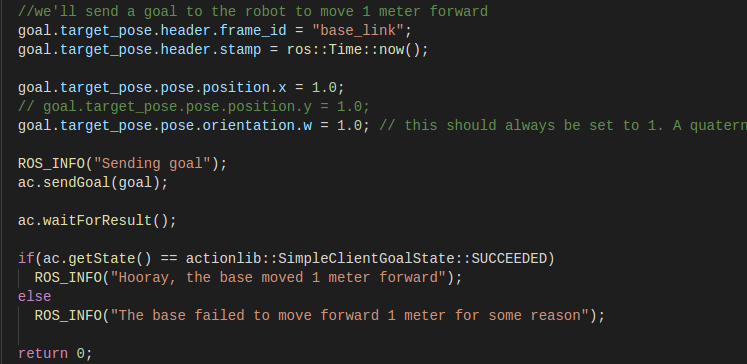
\includegraphics[width=.7\textwidth]{figures/send_goals.png}
	\caption{Implementation of an action to send the robot a goal}
	\label{fig:send_goals}
\end{figure}

The \textbf{goal} object (not visible in the Figure \ref{fig:send_goals}) is of type \textbf{nav{\_}msgs::MoveBaseGoal}, which is the data type used for the \textbf{move{\_}base} to send data. For this specific case I tested the robot to move 1 meter forward, hence the \textbf{x} is set to one. By editing properly the CMakeList an executable is created, under the devel/lib folder, and by \textbf{rosrun} the node, the robot nicely moves one meter forward. 

\vline

By echoing the \textbf{odometry/filtered} topic however, the results in the x-direction are different, as seen in Figure \ref{fig:odom_filt}, and the same holds when echoing the \textbf{amcl{\_}pose} topic, as seen in Figure \ref{fig:amcl_pose}. 

\begin{figure}[!htb]
	\center
	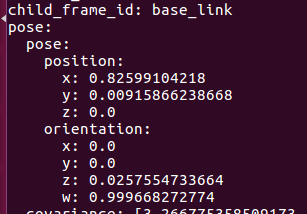
\includegraphics[width=.4\textwidth]{figures/odom_filtered.png}
	\caption{odom filtered}
	\label{fig:odom_filt}
\end{figure}

For both cases the reduction is around \textbf{20 percent} less. I am not sure why now, but it is most probably due to parameters in the \textbf{global and local costmap} and \textbf{amcl.cpp}.

\begin{figure}[!htb]
	\center
	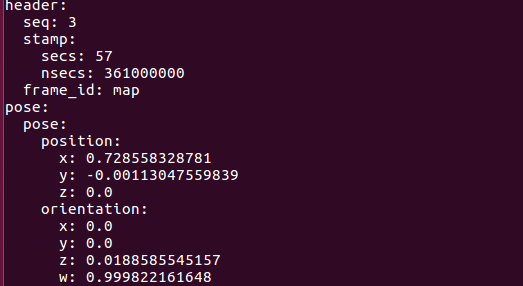
\includegraphics[width=.6\textwidth]{figures/amcl_pose.png}
	\caption{amcl pose topic}
	\label{fig:amcl_pose}
\end{figure}


\section{The Global planner as a reference path} \label{sec:global_planner}

It is possible to define an own Global planner for the robot to follow, as a plugin. This is appended to the \textbf{move{\_}base.launch} file as a parameter, and overrides the functionalities of the already implemented Global planner. What the Global Planner in Figure \ref{fig:global_plann} does is to fill a vector of \textbf{plan} with dummy poses created in the for loop. In this way the robot, once the goal is set, as to follow the path. This however, does not move the robot in any direction autonomously. To do so, the \textbf{next to do} is couple the functionality of Section \ref{sec:move-base} and send an action for each new step goal reached. Currently I am figuring out to do couple those 2 node to work in \textbf{tandem}. 

\vline

As input for the \textbf{new{\_}goal}, instead of single dummy points, I will read coordinates from a .txt file, and save each line in a string. This has been already made in Matlab, and consists of 3 columns and N goals rows. 

\begin{figure}[!htb]
	\center
	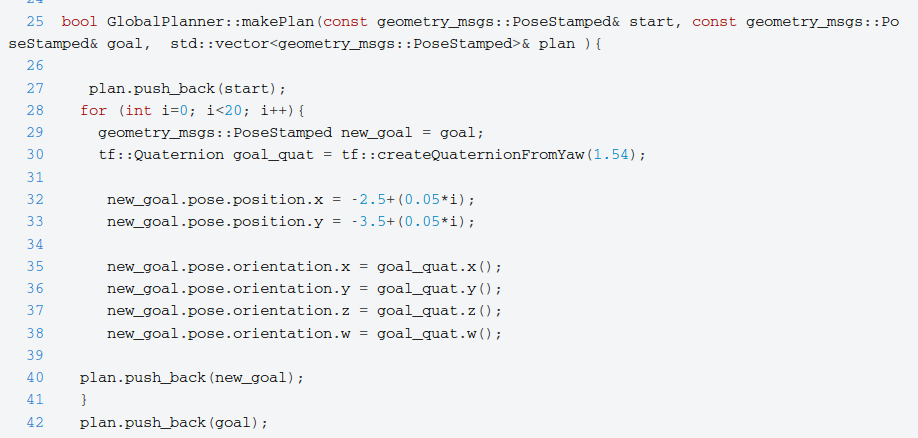
\includegraphics[width=.8\textwidth]{figures/global_planner_ros.png}
	\caption{The simple Global Planner as plugin}
	\label{fig:global_plann}
\end{figure}
















\end{document}



% == TABLE ==
%begin{table}[h!]
 % \centering
  %\caption{Caption for the table.}
 % \label{tab:table1}
 % \begin{tabular}{ccc}
 %   \toprule
  %  Some & actual & content\\
   % \midrule
   % prettifies & the & content\\
   % as & well & as\\
  %  using & the & booktabs package\\
  %   \bottomrule
  %\end{tabular}
%\end{table}


% === ALGORITHM == 

\iffalse % multi-comment tool
\begin{algorithm}[!h]
   \caption{Kirsch, Rohig algorithm}
    \begin{algorithmic}[1]
    	\State $St-1 = St$
        \For{$i = 1$ to $N$} \Comment{With N the number of particles in the filter set by maxparticle parameter}
            \State $Spread $ $particles$ $in$ $the$ $anchorbox$ $with$ $equations$ $1)$ $and$ $2)$ $of$ $[3]$ \Comment{This step is called $Global$ $Localization$}
            
            \State $xt[n] = p(xt|xt-1,ut)$ \Comment{Motion update - sample the particles from the motion update of the robot and move forward to estimate the error model functions}
            
        	\State $wt[n] = p(dnanoLOC|si)*p(dlaser|si)$ \Comment{Measurement update - si are the particles set with i the i-th index}
        	\State $St = St + <xt,wt>$ \Comment{add the state and weight to the total state space}
        	
        	\State $Perform$ $resampling$
        \EndFor
    \State $Return$ $St$

\end{algorithmic}
\end{algorithm}
\fi


\iffalse

\begin{figure}[!htb]
    \centering
    \begin{minipage}{.5\textwidth}
        \centering
        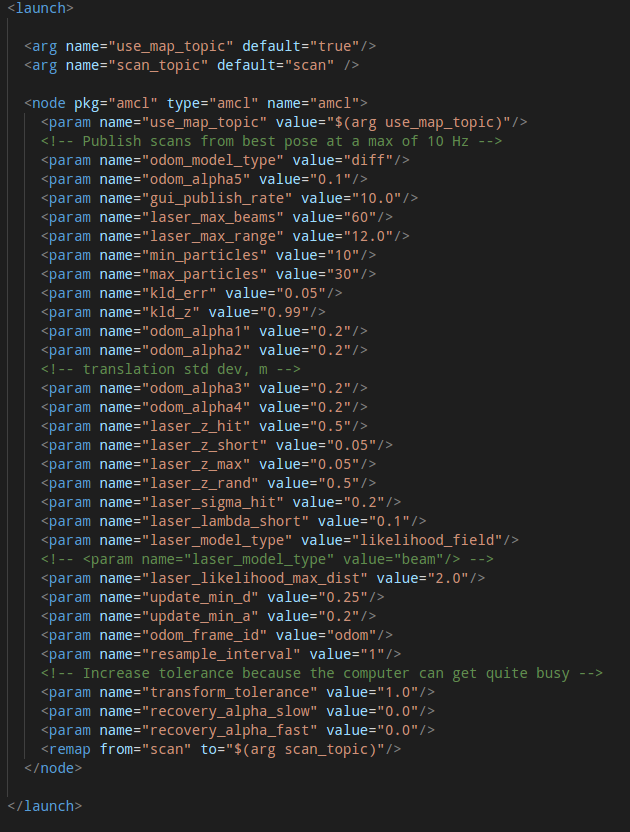
\includegraphics[width=0.7\linewidth, height=0.2\textheight]{figures/amcl_param}
        \caption{The $amcl$ tunable parameters}
        \label{fig:amcl_param}
    \end{minipage}%
    \begin{minipage}{0.5\textwidth}
        \centering
        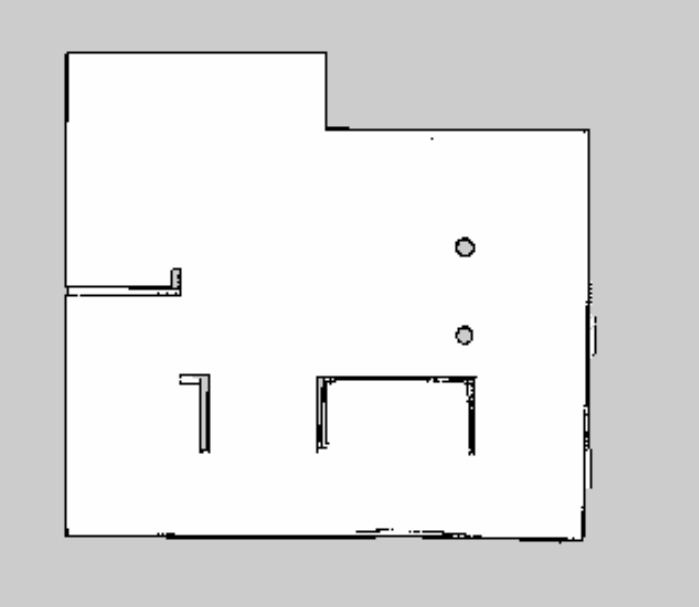
\includegraphics[width=0.7\linewidth, height=0.2\textheight]{figures/my_amcl_gmapping}
        \caption{Result of the Gmapping for the simple indoor environment}
        \label{fig:myamcl_map}
    \end{minipage}
 \end{figure}
 
 
 
 \begin{figure}[!htb]
	\center
	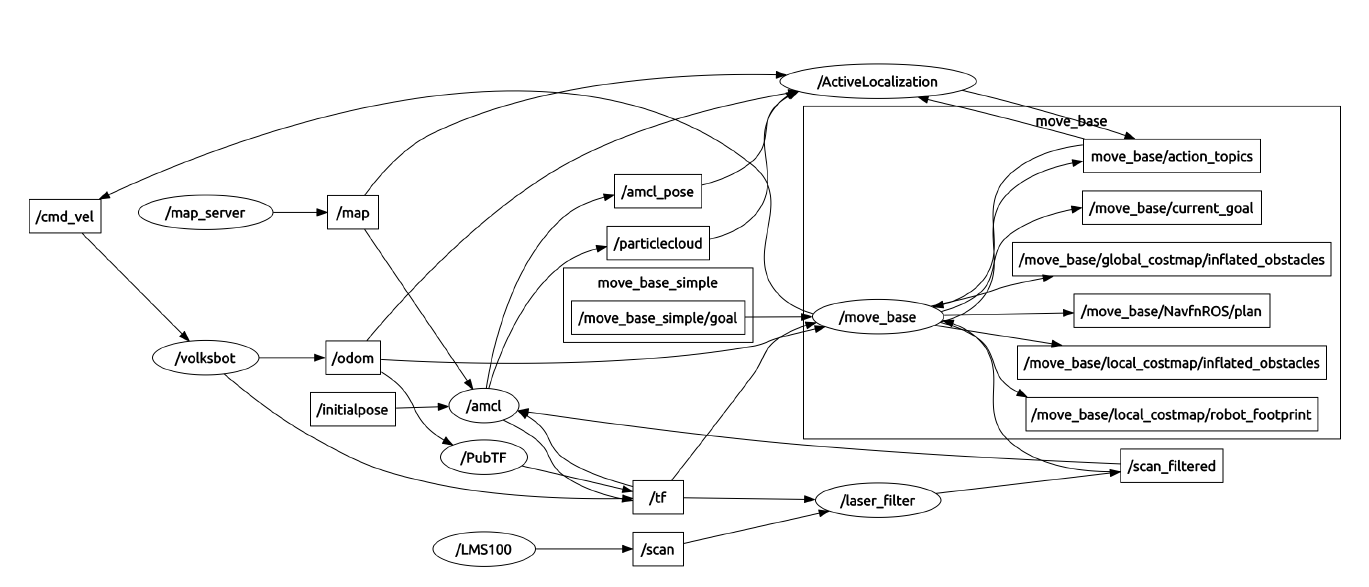
\includegraphics[width=1\textwidth]{figures/active_localization_node.png}
	\caption{An example of an active localization node}
	\label{fig:active_locnode}
\end{figure}


% underscore symbol {\_}


\fi